\section{RESULTS}
Demographics of the 30 respondents are given below:

\begin{itemize}
	\item Role: 47\% Developer, 13 \% Tester, 13\% Business Specialist, 7\% Team Lead, 7\% Project Manager, 3\% Test Manager, 10\% Did not answer
    \item Years in the company: 47\% 0-4 years, 7\% 5-9 years, 13\% 10-14 years, 13\% 15-19 years, 13\% 20 years or more, 7\% Did not answer
    \item Overall work experience in years: 17\% 0-5 years, 20\% 5-10 years, 17\% 10-15 years, 30\% 15-20 years, 10\% more than 20 years, 7\% Did not answer
\end{itemize}

Two of the four interviewees were senior software developers, both with 3 years of working experience in the company. The two others were business architect and tester, both employed in the company for 18 years.

 

 \subsection{Current Development Environment}
The company has been utilizing agile methods for over a decade. They have a company-wide development process based on Scrum. They also utilize Kanban in some of their teams. The company is interested in modern software development approaches such as continuous deployment and DevOps and they are in transition towards utilizing those. However, as the company has thousands of employees in several countries and they are running large customer projects, the transition is not straightforward.
The current approach for software engineering was described in the interviews as follows. Feature requests are gathered and handled by customer support. Development organization gets those as product backlog items and prioritize them based on internal parameters. Development organisation utilizes cloud technologies such as IaaS, PaaS, and SaaS (Infrastructure, Platform, Software as a Service) for build, test, deployment and application management. They use Git for version control. They also do continuous integration but do not run all test to all Git commits. Deployment is done manually by a separate operations organization that is responsible for configuring and setting up production environments. Operations department also takes care or databases, backups of software builds and reversing bad builds in case of errors in new software versions. Deployments to production are typically done once in a month and larger releases are due quarterly.  

\subsection{Challenges in Adopting Continuous Deployment and DevOps}
The interviewed business architect saw the current organizational structure as the main barrier to adopting DevOps. The company has separate development and operations organisations and they have run into difficulties and bureaucracy with utilizing competencies across departments. The business architect gave an example that developers know how to setup a system, but only operations have the rights to perform the setup. 

Interviewed developers mentioned that many of the company's products are running on legacy systems which do not necessarily support continuous development. Changing platforms to such that support a continuous development environment is not feasible. They however implement all new systems development on platforms that support modern software development. They host their new projects on a cloud computing platform and plan to use it increasingly in the future. They have also changed their version control to Git and improved their programming practices and standards to better support continuous development as guided by the cloud computing platform provider.

We asked in the survey how often the respondents experience certain development and deployment related issues in their projects (fig. \ref{fig:percentage_challenges}). "Infrequent releases" and "Time consuming to test" were rather common as 36\% and 28\% of the respondents, respectively, reported experiencing those either "Often" or "Always". The interviewees reported on having quarterly releases and monthly smaller deployments 

\begin{figure}%[H]
\centering
\fbox{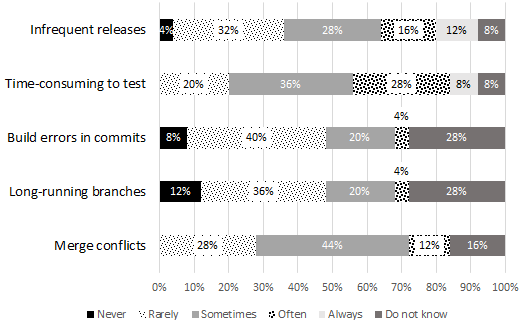
\includegraphics[scale=0.6]{figures/deployment_challenges.png}}
\caption{Frequency of development and deployment related issues as experienced by the survey respondents, N = 30. }
\label{fig:percentage_challenges}
\end{figure}

\begin{figure}%[H]
  \centering
  %\fbox{\includegraphics[scale=0.9]{q_task_prep.PNG}}
  \fbox{\includegraphics[width=0.46\textwidth,height=50mm]{figures/q_task_prep.PNG}}
  \caption{Frequency of task preparation}
  \label{fig:frequency_of_task_preparation}
\end{figure}



The results considering the current state of the pipeline along with improvements is associated with RQ1. These results should give descriptive information about the opinions and actualization of processes in the pipeline.

 (figure \ref{fig:percentage_challenges}). Using continuous testing and continuous deployment from continuous delivery could result in minimizing these challenges. 


The two largest challenges "Time consuming to test" and "Infrequent releases" (figure \ref{fig:percentage_challenges}) are also the ones, which most respondents agreed on could be solves by continuous methods, continuous deployment and continuous testing respectively (figure \ref{fig:percentage_minimizing_challenges}). 
A large part of the respondents had answered "do not know" on which continuous methods could minimize derlivery challenges, which might be due to lack of knowledge on continuous methods or confusion on the question formulation (figure \ref{fig:percentage_minimizing_challenges}).


\begin{figure}%[H]
\centering
\fbox{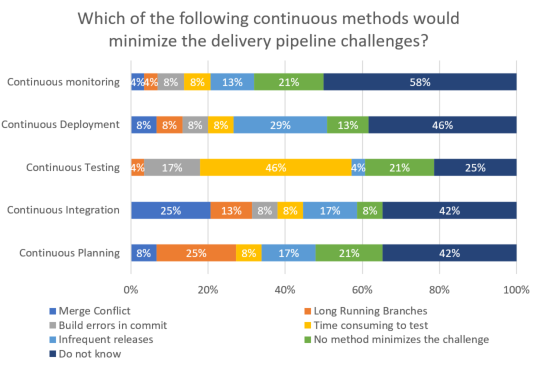
\includegraphics[scale=1.2]{figures/q_challenges_continuous.PNG}}
\caption{Opinions on how continuous methods can minimize  development challenges}
\label{fig:percentage_minimizing_challenges}
\end{figure}


\subsection{Reusable code}
The results concerning reusable code is a topic mainly initiated by the company, that will provide information to answering RQ2 about what contributes to better reusable coding.

% Note til figur: folk vil ikke have education (men ved folk nok om principper?)
\begin{figure}%[H]
\centering
\fbox{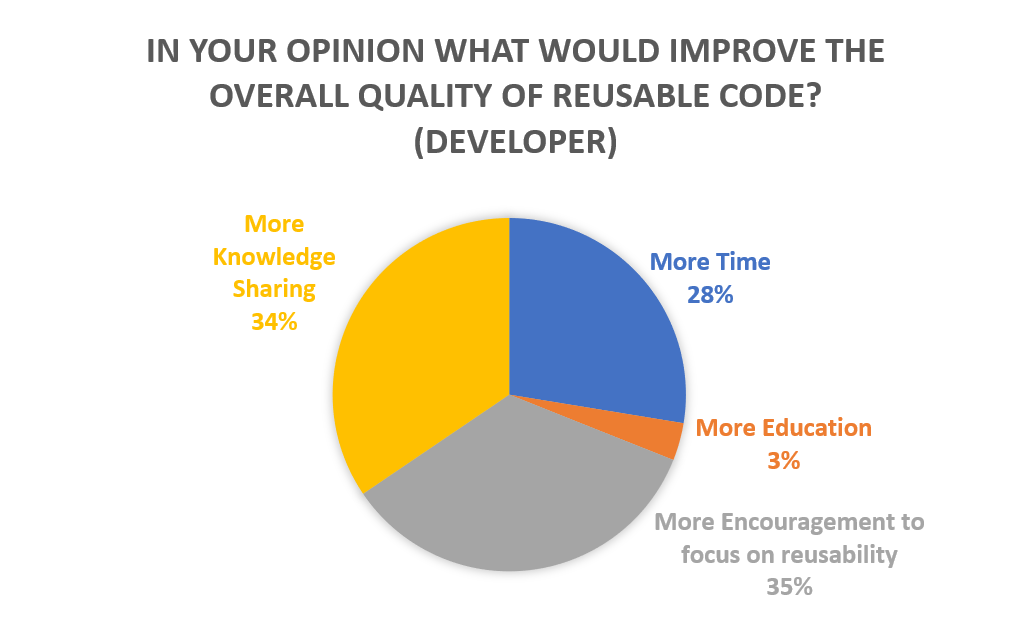
\includegraphics[scale=1.1]{figures/q_reusable_code.PNG}}
\caption{Opinions on improvements regarding reusable code (Only developers, N = 14)}
\label{fig:opinion_of_improvement_to_reusable_code}
\end{figure}

The respondents would like more encouragement to focus on reusability, followed by more knowledge sharing in the teams (figure \ref{fig:opinion_of_improvement_to_reusable_code}). The respondents would also like more time to find and applying reusable code. However, the respondents did not believe that they needed more education on reusable code principles.  

% Note til figur: Over 25% bruger enten ingen principper eller ved ikke (se nærmere om "ved ikke" i næste tabel)
\begin{figure}%[H]
\centering
\fbox{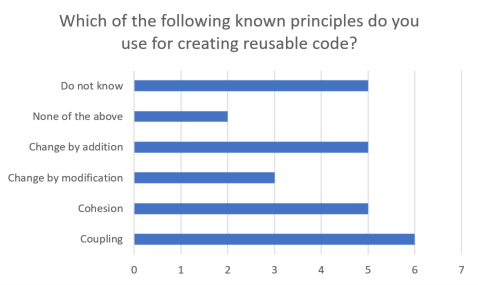
\includegraphics[scale=1.1]{figures/q_reusable_code_2.PNG}}
\caption{Usage of reusable code principles (N = 15)}
\label{fig:usage_of_reusable_code_principles}
\end{figure}

13.3\% of the respondents do not make use of the listed known code reusable code principles and 33.3\% were not familiar with the principles (figure \ref{fig:usage_of_reusable_code_principles}). However the remaining 53.3\% of respondents made use of known reusable code principles. This indicates that the respondents may benefit from more education on reusable code even though it was contradictory with the results of figure \ref{fig:opinion_of_improvement_to_reusable_code}.


From 30 responses 35.5\% agreed that they do "Task elaboration" (figure \ref{fig:frequency_of_task_preparation}). Further task elaboration might be time consuming and also might indicate that a given task might not be informative enough for the respondents. The second and third most chosen actions were "Find similar solutions locally" and "Investigate existing customer solution" respectively, which indicates useful information for RQ2, where the code reusability was highlighted. It can also be seen that "Modeling the solution" was very low which references to RQ3 about system design.

\iffalse
\begin{itemize}
  \item There was asked how the employee prioritized the different software processes to know if everyone agrees about the pipeline or if there were any confusion. Through this table it could be seen that the respondents all agree with how to prioritize the processes in the software pipeline. One can discuss that design and implementation could with advantages be switched around which also can be seen in the box plot below. 
  \item Point 2
\end{itemize}
\fi